\chapter{Requirements Engineering}
\label{ch:requirements}

If you build the wrong system, no amount of clever design will save it. Requirements engineering (RE) is the disciplined process of discovering, documenting, and validating \emph{what} the system must do and \emph{how well} it must do it. Errors here are the most expensive category of defect---studies attribute over $40\%$ of rework cost to requirements issues.

\section{Requirements Basics}

\begin{definition}[Requirement]
A condition or capability needed by a user to solve a problem or achieve an objective; a condition or set of conditions that must be met by the system to satisfy a contract, standard, or specification.
\end{definition}

Two orthogonal dimensions classify every requirement:

\begin{itemize}
    \item \textbf{Functional (FR)} --- \emph{what} the system does: features, behaviours, data transformations, business rules. Testable by observing outputs for given inputs.
    \item \textbf{Non-functional (NFR)} --- \emph{how well} the system does it: qualities, constraints, compliance, and emergent properties. Often cross-cutting and harder to test.
    \item \textbf{Domain requirements} --- constraints from the application domain (e.g., ``student GPA is on a 5.0 scale''), which may be functional or non-functional.
\end{itemize}

\begin{example}
For an online exam system: ``The system shall auto-grade MCQ answers and display the score'' is functional; ``The system shall support 5{,}000 concurrent examinees with 99.9\% uptime and grade within 2~seconds'' combines performance, scalability, and availability NFRs.
\end{example}

A common pitfall is stating solutions instead of needs: ``The system shall use MySQL'' is a design constraint, not a requirement, unless the stakeholder truly mandates it. Good requirements are abstract enough to leave design freedom.

\section{FURPS+ for Non-Functional Requirements}

The FURPS+ taxonomy (Grady, HP) ensures NFR coverage is systematic rather than ad hoc:

\begin{figure}[h]
\centering
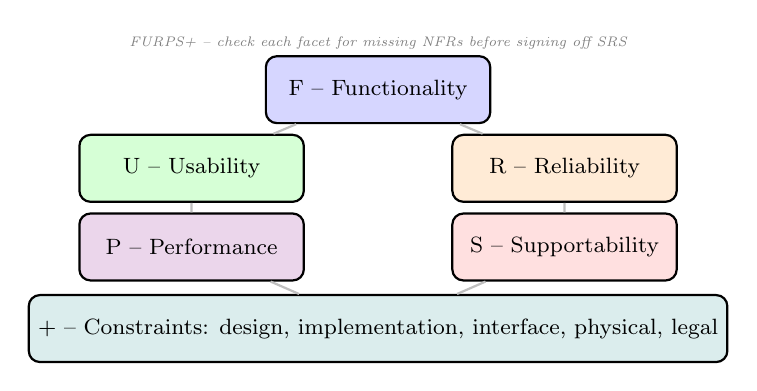
\begin{tikzpicture}[scale=0.74, every node/.style={font=\footnotesize}]
  \tikzstyle{cat}=[draw,rounded corners,minimum width=2.85cm,minimum height=0.85cm,align=center,thick]
  \node[cat,fill=blue!16] (f) at (0,3.2) {F -- Functionality};
  \node[cat,fill=green!16] (u) at (-3.2,1.85) {U -- Usability};
  \node[cat,fill=orange!16] (r) at (3.2,1.85) {R -- Reliability};
  \node[cat,fill=violet!16] (p) at (-3.2,0.5) {P -- Performance};
  \node[cat,fill=red!12] (s) at (3.2,0.5) {S -- Supportability};
  \node[cat,fill=teal!14] (plus) at (0,-0.9) {+ -- Constraints: design, implementation, interface, physical, legal};
  \draw[thick,gray!50] (f) -- (u) -- (p) -- (plus) -- (s) -- (r) -- (f);
  \node[font=\tiny\itshape,gray] at (0,4.0) {FURPS+ -- check each facet for missing NFRs before signing off SRS};
\end{tikzpicture}
\caption{FURPS+ model for eliciting non-functional requirements systematically. Each letter prompts a checklist of quality attributes.}
\end{figure}

Each facet prompts concrete questions. \emph{Usability}: learnability, accessibility (WCAG), localisation. \emph{Reliability}: MTBF, recoverability, fault tolerance. \emph{Performance}: throughput, latency percentiles, capacity. \emph{Supportability}: maintainability, configurability, installability. The ``+'' captures constraints such as ``must run on Android~12+'', ``must comply with PDPA'', or ``must integrate with the university SSO''.

Well-formed requirements follow \textbf{SMART} and \textbf{INVEST} (for stories): Specific, Measurable, Achievable, Relevant, Traceable. ``System should be fast'' fails; ``95th-percentile API latency $<$ 300~ms under 1{,}000~rps sustained for 10~minutes'' passes because it is verifiable.

\section{Requirements Engineering Process}

\begin{enumerate}
    \item \textbf{Elicitation} --- interviews, workshops, observation, questionnaires, prototyping, brainstorming, and analysis of existing systems. The goal is to surface both stated and tacit needs.
    \item \textbf{Analysis \& negotiation} --- resolve conflicts (customer wants X, operator wants not-X), prioritise via MoSCoW (Must/Should/Could/Won't), detect ambiguity and incompleteness.
    \item \textbf{Specification} --- document in an SRS (Software Requirements Specification) with unique IDs, priorities, sources, and verification methods.
    \item \textbf{Validation} --- reviews, walkthroughs, prototypes, and traceability checks to ensure requirements are correct, complete, and consistent.
    \item \textbf{Management} --- version, trace, and control change requests; every change is impact-analysed.
\end{enumerate}

Stakeholders include end users, customers (who pay), developers, testers, operators, and regulators. Missing a stakeholder class is a classic failure mode---operators care about deployability, regulators about compliance, and both are often forgotten until late.

\begin{figure}[h]
\centering
\begin{tikzpicture}[scale=0.72, every node/.style={font=\scriptsize}]
  \tikzstyle{reqstep}=[draw,rounded corners,fill=blue!10,minimum width=2.6cm,minimum height=0.9cm,align=center,thick]
  \node[reqstep,fill=green!14] (e) at (0,0) {Elicitation};
  \node[reqstep,fill=orange!14] (a) at (3.5,0) {Analysis};
  \node[reqstep,fill=violet!14] (s) at (7.0,0) {Specification};
  \node[reqstep,fill=red!12] (v) at (10.5,0) {Validation};
  \draw[-{Stealth},thick] (e) -- (a);
  \draw[-{Stealth},thick] (a) -- (s);
  \draw[-{Stealth},thick] (s) -- (v);
  \draw[-{Stealth},thick,dashed,gray,bend left=18] (v) to (a);
  \draw[-{Stealth},thick,dashed,gray,bend left=18] (a) to (e);
  \node[draw,fill=yellow!15,rounded corners,font=\tiny,align=center] at (5.25,-1.4) {Management (versioning, traceability, change control)\\runs continuously across all phases};
  \draw[dashed,gray] (5.25,-0.7) -- (5.25,-1.05);
\end{tikzpicture}
\caption{RE process is iterative with feedback loops; management activities span the entire lifecycle.}
\end{figure}


\section{Requirement Prioritisation and Negotiation}

Not all requirements are equal. MoSCoW (Must, Should, Could, Won't) provides a simple prioritisation that forces stakeholders to make trade-offs. Kano analysis adds nuance by distinguishing basic needs (dissatisfiers if absent), performance needs (linear satisfaction), and delighters (non-linear upside). A requirement that is a delighter for one stakeholder may be a basic need for another -- negotiation is therefore central to RE.

Techniques for resolving conflicts include win-win negotiation (Boehm), where each stakeholder's win conditions are made explicit and negotiated until every party's must-haves are satisfied, and cost-value prioritisation where each requirement is scored on business value and implementation cost, then plotted to identify high-value, low-cost quick wins versus expensive, low-value items to defer or drop.

\section{Common Pitfalls}

Requirements errors follow predictable patterns: \emph{ambiguity} (``fast'' without quantification), \emph{incompleteness} (missing exception flows), \emph{inconsistency} (two requirements contradict), \emph{infeasibility} (violates physics or budget), and \emph{premature design} (stating a solution rather than a need). Inspections using checklists derived from FURPS+ and SMART catch many of these before they become rework.

\section{Use Cases and User Stories}

\subsection{Use-Case Diagrams}

A use case captures a goal-oriented interaction between actors and the system. The diagram shows the system boundary, actors (stick figures), use cases (ellipses), and relationships: \texttt{include} (mandatory sub-flow), \texttt{extend} (optional/alternative flow), and generalisation.

\begin{figure}[h]
\centering
\begin{tikzpicture}[scale=0.74, every node/.style={font=\footnotesize}]
  \draw[thick,rounded corners,fill=blue!4] (-1.3,-2.3) rectangle (4.3,2.7);
  \node[font=\scriptsize\itshape] at (1.5,2.95) {Online Exam System};
  \tikzstyle{uc}=[draw,ellipse,fill=orange!16,minimum width=2.5cm,minimum height=0.9cm,align=center,thick]
  \node[uc] (uc1) at (1.5,1.9) {Take Exam};
  \node[uc] (uc2) at (1.5,0.65) {Auto-Grade};
  \node[uc] (uc3) at (1.5,-0.7) {View Results};
  \node[uc] (uc4) at (1.5,-1.65) {Manage Questions};
  % actors
  \node[draw,circle,fill=green!15,minimum size=0.7cm,thick] (s) at (-3.2,0.9) {};
  \node[below=0.05cm of s,font=\scriptsize] {Student};
  \draw[thick] (s) -- ++(0,-0.45);
  \node[draw,circle,fill=violet!15,minimum size=0.7cm,thick] (t) at (-3.2,-1.2) {};
  \node[below=0.05cm of t,font=\scriptsize] {Instructor};
  \draw[thick] (t) -- ++(0,-0.45);
  % relations
  \draw[thick] (s) -- (uc1);
  \draw[thick] (s) -- (uc3);
  \draw[thick] (t) -- (uc4);
  \draw[thick] (t) -- (uc3);
  \draw[dashed,->,thick,gray] (uc1) -- (uc2) node[midway,above,font=\tiny] {$\langle\langle$include$\rangle\rangle$};
  \node[font=\tiny,gray,align=left] at (6.2,0.6) {extend: e.g.,\\``Flag for review''};
  \draw[dashed,->,gray] (5.3,0.2) -- (uc1.east);
\end{tikzpicture}
\caption{Use-case diagram for an online exam system -- actors, boundary, and an include relationship (Take Exam always triggers Auto-Grade).}
\end{figure}

A use-case \emph{specification} details preconditions, main flow (numbered steps), alternative flows, exceptions, and postconditions. For \emph{Take Exam}, the main flow has seven steps from authentication through submission and confirmation; alternative flow 3a handles network timeout with retry, and 5a handles out-of-time auto-submit.

\subsection{User Stories and Acceptance Criteria}

Agile teams often prefer the terse format: \emph{As a $\langle$role$\rangle$ I want $\langle$goal$\rangle$ so that $\langle$benefit$\rangle$}. Each story carries acceptance criteria in Given/When/Then form and is sized to fit one iteration (INVEST: Independent, Negotiable, Valuable, Estimable, Small, Testable).

\begin{lstlisting}[language=Python,caption={Acceptance criteria as executable specification (Gherkin-style).}]
# Story: As a student I want auto-grading so that I get instant feedback
# Scenario: MCQ auto-grading
#   Given I have submitted answers for 10 MCQs
#   When the grading service runs
#   Then each correct answer scores 1 point
#   And total score is displayed within 2 seconds
def test_mcq_grading():
    answers = ["A","B","A","C","D","A","B","C","A","D"]
    key     = ["A","B","A","C","D","A","B","C","A","D"]
    assert grade(answers, key) == 10
    assert grade_latency_ms(answers, key) < 2000
\end{lstlisting}

Stories are not replacements for use cases at scale; they complement them. A common pattern is to start with use cases for scope, then slice each into stories for iterative delivery.


\section{Requirements Validation Techniques}

Validation answers ``are we building the right system?'' Techniques include formal inspections (Fagan), peer reviews, prototyping (throwaway vs.\ evolutionary), and model checking of state-based requirements. A lightweight but effective method is the \emph{requirements walkthrough}: the analyst walks stakeholders through each requirement with concrete scenarios, often revealing hidden assumptions. Traceability matrices are validated by ensuring every requirement has at least one test and every test traces to a requirement.

\section{SRS and Traceability}

An SRS (IEEE~830 style) organises requirements hierarchically with unique IDs (REQ-001), priority (MoSCoW), source stakeholder, and verification method (test, inspection, demonstration). A \emph{traceability matrix} links each requirement to design elements, code modules, and tests---so no requirement is lost and no code is unjustified. When a requirement changes, the matrix instantly reveals the blast radius.


\section{Elicitation Techniques Compared}

\begin{table}[h]
\centering\small
\begin{tabular}{@{}lccp{4.2cm}@{}}
\toprule
Technique & Richness & Cost & Best when \\ \midrule
Interview & High & Medium & Stakeholders are accessible, domain is tacit \\
Workshop & High & High & Conflicts need resolution quickly \\
Observation & Medium & Low & Users cannot articulate workflow \\
Questionnaire & Low & Low & Large, distributed population \\
Prototyping & High & Medium--High & Requirements are uncertain or UI-heavy \\
\bottomrule
\end{tabular}
\caption{Selecting elicitation techniques -- no single technique suffices; combine at least two.}
\end{table}

Triangulation (using multiple techniques) catches what any single method misses. An interview may reveal that ``students want faster feedback,'' but only observation shows that the bottleneck is manual grade entry, not grading logic -- pointing to a workflow requirement rather than an algorithmic one.


\begin{remark}
Non-functional requirements often dominate architecture: ``support 10k concurrent users'' drives caching, sharding, and load-balancing decisions far more than any single functional requirement.
\end{remark}

\section{Exercises}

\begin{exercise}
Classify each as FR or NFR and justify: (a) ``System shall encrypt passwords with bcrypt'', (b) ``System shall allow password reset via email'', (c) ``Password-reset email shall arrive within 60~s for 99\% of requests''. Which FURPS+ facet does each NFR belong to?
\end{exercise}

\begin{exercise}
Write a full use-case specification (preconditions, main flow 5--7 steps, two alternative flows, postconditions) for ``Borrow Book'' in a library system with Student and Librarian actors. Include an include relationship for ``Check Overdue''.
\end{exercise}

\begin{exercise}
Convert the use case in the previous exercise into three user stories with Given/When/Then acceptance criteria. Discuss what is gained and lost in the conversion and when you would keep the use-case form.
\end{exercise}

\begin{exercise}
A stakeholder says ``The system should be user-friendly and handle many users.'' Rewrite this as two SMART requirements and explain how you would validate each (inspection, test, or demonstration).
\end{exercise}

\begin{exercise}
Draw a traceability fragment linking REQ-007 ``Auto-grade within 2~s'' to one design component, one code module, and one test case. Explain how the matrix helps when a change request tightens the limit to 1~s.
\end{exercise}
